\documentclass[12pt]{article}
\usepackage{verbatim}
\usepackage[dvips]{epsfig}
\usepackage{color}
\usepackage{lineno}
\usepackage{url}
\usepackage[colorlinks=true]{hyperref}

\begin{document}

\section*{GENESIS: Documentation}

{\bf Related Documentation:}
% start: userdocs-tag-replace-items related-cbi-architecture
% end: userdocs-tag-replace-items related-cbi-architecture

%\section*{Multi-Scale Modeling within the CBI Simulator Framework}

\begin{flushleft}
{\Large
\textbf{Multi-Scale Modeling within the CBI Simulator Framework}
}
% Insert Author names, affiliations and corresponding author email.
\\
Hugo Cornelis$^{1,^\ast}$, 
Allan D. Coop$^{2}$,
Armando L. Rodriguez$^{3}$, 
Dave Beeman$^{4}$,
James M. Bower$^{5}$.
\\
\vspace*{5mm}
\begin{small}
{1.} Cornelis H. Department of Neurophysiology, Catholic University of Leuven, Leuven, 3000, Belgium
\\
{2.} Coop A. D. Director of Flight Simulation, Merindah Energy.
\\
{3.} Rodriguez A. L. Research Imaging Institute, University of Texas Health Science Center at San Antonio, San Antonio, TX, United States
\\
{4.} Beeman D. Department of Electrical, Computer, and Energy Engineering, University of Colorado, Boulder, CO 80309
\\
{5.} Bower J. M. Research Imaging Institute, University of Texas Health Science Center at San Antonio, San Antonio, TX, United States
\\
$^\ast$ E-mail: Corresponding Author Hugo.Cornelis@gmail.com
\end{small}
\end{flushleft}

\newpage

\tableofcontents

\newpage

\section{Results}

\subsection{The Neurospaces Description Format}

The {\bf Model Container}'s {\it Neurospaces Description Format} ({\it
  NDF}) file format was originally designed as a file-based
user-editable declarative interface to the {\bf HSolve} method in
GENESIS-2 in 1999\cite{cornelis03:_neuros}.  In that same year it was
expanded with single neuron and network modeling capabilities.

The file format is indicated by the {\tt .ndf} file name extension and
integrates and extends the previous GENESIS {\tt .p} and {\tt .g}
declarative file formats.  {\bf NDF} files are purely declarative in
nature such that they may be stored in a model database. In an {\bf
  NDF} file, a model exists as a hierarchy of tokens, each
representing a biological component.  Each component is a physical
process and can have parameters and shared variables.

\subsubsection*{Overview of a {\bf NDF} File}
\label{sec:overview-ndf-file}
%We now introduce the basic parts of a simple {\bf NDF} file that defines a single compartment neuron containing classical Hodgkin-Huxley descriptions of $Na$ and $K$ channels.
A {\bf NDF} file contains four sections. These sections are not necessarily
filled, but they must be present in the given order.  A {\bf NDF} file has
the following general form which we describe in more detail below.

\begin{center}
 \begin{linenumbers}
 % \begin{boxedminipage}{13cm}
\begin{verbatim}
    #!/usr/local/bin/neurospacesparse
    //-*- NEUROSPACES -*-

    // default location for file comments

    NEUROSPACES NDF

    IMPORT
        FILE <namespace> "<directorypath>/<filename.ndf>"
         . . . <other files may be imported as required>
    END IMPORT

    PRIVATE_MODELS
        ALIAS <namespace>::/<source label> <target label> END ALIAS
            . . . <other aliases may be defined as required>
    END PRIVATE_MODELS

    PUBLIC_MODELS
        CELL <morphology name>
            SEGMENT_GROUP segments
                . . . <morphological details>
            END SEGMENT_GROUP
        END CELL
    END PUBLIC_MODELS
\end{verbatim}
%  \end{boxedminipage}
\end{linenumbers}
\end{center}

\paragraph*{Header Section}
The header, which runs from lines 1--6 in the previous example, must
always be present and must always start with the interpreter sequence
giving the system specific absolute path to the NMC executable:
\begin{verbatim}
    #!/usr/local/bin/neurospacesparse
\end{verbatim}
This is followed by two declarations on separate lines. 
\begin{verbatim}
    //-*- NEUROSPACES -*-
    
    NEUROSPACES NDF
    \end{verbatim}
The first (optional) declaration (line 2) flags an appropriate major
mode and keyword highlighting for Emacs and XEmacs
editors\footnote{The Neurospaces Emacs major mode is bundled with the
  NMC package.}, the second (line 6) identifies the type of file, here
a {\bf NDF} file.

\paragraph*{Import Section}
This section (lines 8--11) uses the {\tt FILE} keyword to declare
dependencies on other {\bf NDF} files, e.g.
\begin{verbatim}
    IMPORT
        FILE <namespace> "<path>/<fname>.ndf"
    END IMPORT
\end{verbatim}

To simplify model development, GENESIS allows construction of {\bf
  NDF} files that define different components of a model.  These files
may be thought of as \emph{library} files.  To expedite model
development, all {\bf NDF} files can be shared by being imported into
other {\bf NDF} files.

\paragraph*{Private Model Section}
These are models (lines 13--16) that are private to the {\bf NDF} file
that contains them.  They may depend on imported public models of
other files or be hard coded.

\paragraph*{Public Model Section}
These models (lines 18--24) are visible to the {\bf NDF} files into
which they are imported.  Typically, for example, a neuron morphology
would be located here.  Public models may depend on private models or
be hard coded.

\subsubsection*{Summary}
One important feature of a {\bf NDF} file is that it can contain
either a single model or a library of models that represent different
levels of neuronal morphology and/or electrophysiological function.
This supports the modular construction of a model as a {\bf NDF} file
can depend on other {\bf NDF} files, i.e. the models declared in a
{\bf NDF} file can be ``private'' to that file, or ``public'' and
available to other {\bf NDF} files.

As an example, if a first file is dependent on a second file, only the
public files of the second file can be reused to build more
complicated models in the first file. This mechanism prevents the use
of certain (private) components, while allowing reuse of other
(public) components.


\subsubsection*{Physical Processes and Model Variables}

Mathematical models can be used to describe physical processes that underly the functional activity
of biological entities by associating the physical
processes with parameters (fixed during a simulation) and variables
(computed during a simulation).

As an example, a synaptic current is commonly modeled using a
second-order differential equation:
\begin{equation}
  \label{eq:second-order-synchan}
  G'' + \alpha G' + \beta G = S
\end{equation}
with $S = \delta(t - t_1) + \cdots + \delta(t - t_N)$.

In computational neuroscience the right-hand side of this equation
corresponds to the level of synaptic activation delivered by spikes
arriving at times $t_i$.

Assuming the initial values $G(0) = 0$ and $G'(0) = 0$, the solution
to this equation is a dual-exponential equation:
\begin{equation}
  \label{eq:dual-exponential}
  G(t) = \frac{\tau_1\tau_2}{\tau_1 - \tau_2}
  \cdot (\mathrm{e}^{\frac{-t}{\tau_1}} - \mathrm{e}^{\frac{-t}{\tau_2}})
\end{equation}
with $\alpha = \frac{\tau_1 + \tau_2}{\tau_1 \tau_2}$ and $\beta =
\frac{1}{\tau_1 \tau_2}$.
%\begin{equation}
%  \label{eq:simple-spatial-cable}
%  \frac{a}{2R_a}\frac{\partial^2V}{\partial x^2} = C_m \frac{\partial V}{\partial t} + \frac{V}{R_m}
%  + I_{\mathrm{HH}} + I_{\mathrm{syn}}
%\end{equation}
This equation has two parameters {\tt TAU1} and {\tt TAU2}, sometimes
called the rise and decay time constants, respectively.  Assigning
values to the two parameters, this can be expressed in the \href{../ndf-file-format/ndf-file-format.tex}{\bf NDF\,File\,Format}
as:
%EQUATION_EXPONENTIAL exp2

%  ...
\begin{verbatim}
  PARAMETERS
    PARAMETER ( TAU1 = 0.50e-3 ),
    PARAMETER ( TAU2 = 1.20e-3 )
  END PARAMETERS
\end{verbatim}
%END EQUATION_EXPONENTIAL

When one biological entity modulates the behavior of another,
their physical processes share one or more variables.  In the case of
a synaptic channel the incoming spikes raise the neurotransmitter
concentration level in the synaptic cleft, which then modulates total
ionic conductance through channels in the post-synaptic membrane.  The NDF file format expresses the
neurotransmitter concentration level as {\tt activation} and
conductance as {\tt G}.  As these variables  are shared they must be declared using
the {\tt BINDABLES} keyword:
\begin{verbatim}
  BINDABLES
    INPUT activation, OUTPUT G
  END BINDABLES
\end{verbatim}
Assuming a synapse is present under the label {\tt ../synapse}, its
activation level can be bound to the channel activation level using a
{\tt BINDINGS} clause:
\begin{verbatim}
  BINDINGS
    INPUT ../synapse->activation
  END BINDINGS
\end{verbatim}

Putting everything together using the {\tt EQUATION\_EXPONENTIAL}
token to represent the dual-exponential equation, we get the NDF
snippet that defines a model's component with name 'exp2':
\begin{verbatim}
EQUATION_EXPONENTIAL exp2
  BINDABLES
    INPUT activation, OUTPUT G
  END BINDABLES
  BINDINGS
    INPUT ../synapse->activation
  END BINDINGS
  PARAMETERS
    PARAMETER ( TAU1 = 0.50e-3 ),
    PARAMETER ( TAU2 = 1.20e-3 )
  END PARAMETERS
END EQUATION_EXPONENTIAL
\end{verbatim}

In this example, the order of the clauses of {\tt BINDABLES}, {\tt
  BINDINGS} and {\tt PARAMETERS} was chosen for readibility.  
{\bf Note:} Neither the NDF file format nor
the \href{../model-container/model-container.tex}{\bf Model\,Container}
makes a syntactical distinction between the variables and parameters of a
physical process.

The NDF format supports an extensible set of tokens including {\tt
  SEGMENT}, {\tt CHANNEL}, {\tt CELL}, {\tt POPULATION}, {\tt
  PROJECTION}, {\tt NETWORK} and many more that allow the construction of
models ranging from subcellular dynamics up to the network level.


\subsection{Interactive Query and Simulation}

The {\bf G-Shell} integrates other G-3 components and makes their
functions available through an interactive environment available from
a command line.  Coded in Perl, the {\bf G-Shell} is a communication
abstraction layer for the {\bf Model Container}, {\bf Heccer}, {\bf
  SSP}, {\bf DES} and the {\bf Studio}.  After the {\bf G-Shell} has
been started from a system shell with
\begin{verbatim}
   genesis-g3
\end{verbatim}
%the list of loaded software components can be printed to the screen
%with the command:

%\begin{verbatim}
%   list components
%\end{verbatim}

%Each loaded software component will be shown with associated status
%information that helps diagnose possible problems.  For example, after
%correct initialization of the {\bf Model Container} the status
%information appears as:

%\begin{verbatim}
%  model-container:
%    description: internal storage for neuronal models
%    integrator: Neurospaces::Integrators::Commands
%    module: Neurospaces
%    status: loaded
%    type:
%      description: intermediary
%      layer: 2
%\end{verbatim}

Integration of the {\bf G-Shell} with the {\bf Model Container} allows
for real-time analysis of the quantitative and structural aspects of a
neuronal morphology.  The library of model components that is
installed with the {\bf Model Container} provides a definition of a
model Purkinje cell in the file {\it cells/purkinje/edsjb1994.ndf}.
The command:
\begin{verbatim}
   ndf_load cells/purkinje/edsjb1994.ndf
\end{verbatim}
makes this model Purkinje cell available for interactive analysis.
Similar commands exists or are in development for backward-compatible
loading of GENESIS-2 SLI scripts ({\it sli\_load} or to interface with
the PyNN network modeling environment ({\it
  pynn\_load})\cite{davison08:_pynn}.

%Given the name of one of its dendritic segments, the number of branch
%points between the segment and the soma can be determined. After
%indicating with the command {\it morphology\_summarize} which paths of
%the dendritic tree to examine, the parameter {\tt
%  SOMATOPETAL\_BRANCHPOINTS} contains the result, which can be
%obtained with:

%\begin{verbatim}
%   morphology_summarize /Purkinje
%   show_parameter /Purkinje/segments/b1s06[182] SOMATOPETAL_BRANCHPOINTS
%\end{verbatim}

If a dendritic segment contains a synaptic channel, it can be
stimulated with a precomputed spike train stored in a file named, for
example, {\it event\_data/events.yml}:

\begin{verbatim}
   set_runtime_parameter /Purkinje/segments/b1s06[182]/Purkinje_spine_0/head/par/synapse
      EVENT_FILENAME ``event_data/events.yml''
\end{verbatim}

Finally, following the addition of an output for the somatic membrane
potential:
\begin{verbatim}
   add_output /Purkinje/segments/soma Vm
\end{verbatim}
A simulation can then conveniently be started using:
\begin{verbatim}
   run /Purkinje 0.1
\end{verbatim}
This simulation produces the somatic response to the given dendritic
stimulus in a file named, by default, {\it /tmp/output}.

To query the parameters of the stimulated compartment the model can
then be analyzed using the graphical front-end of the {\bf Studio}
with the command:

\begin{verbatim}
   explore
\end{verbatim}

\begin{figure}[ht]
  \begin{center}
    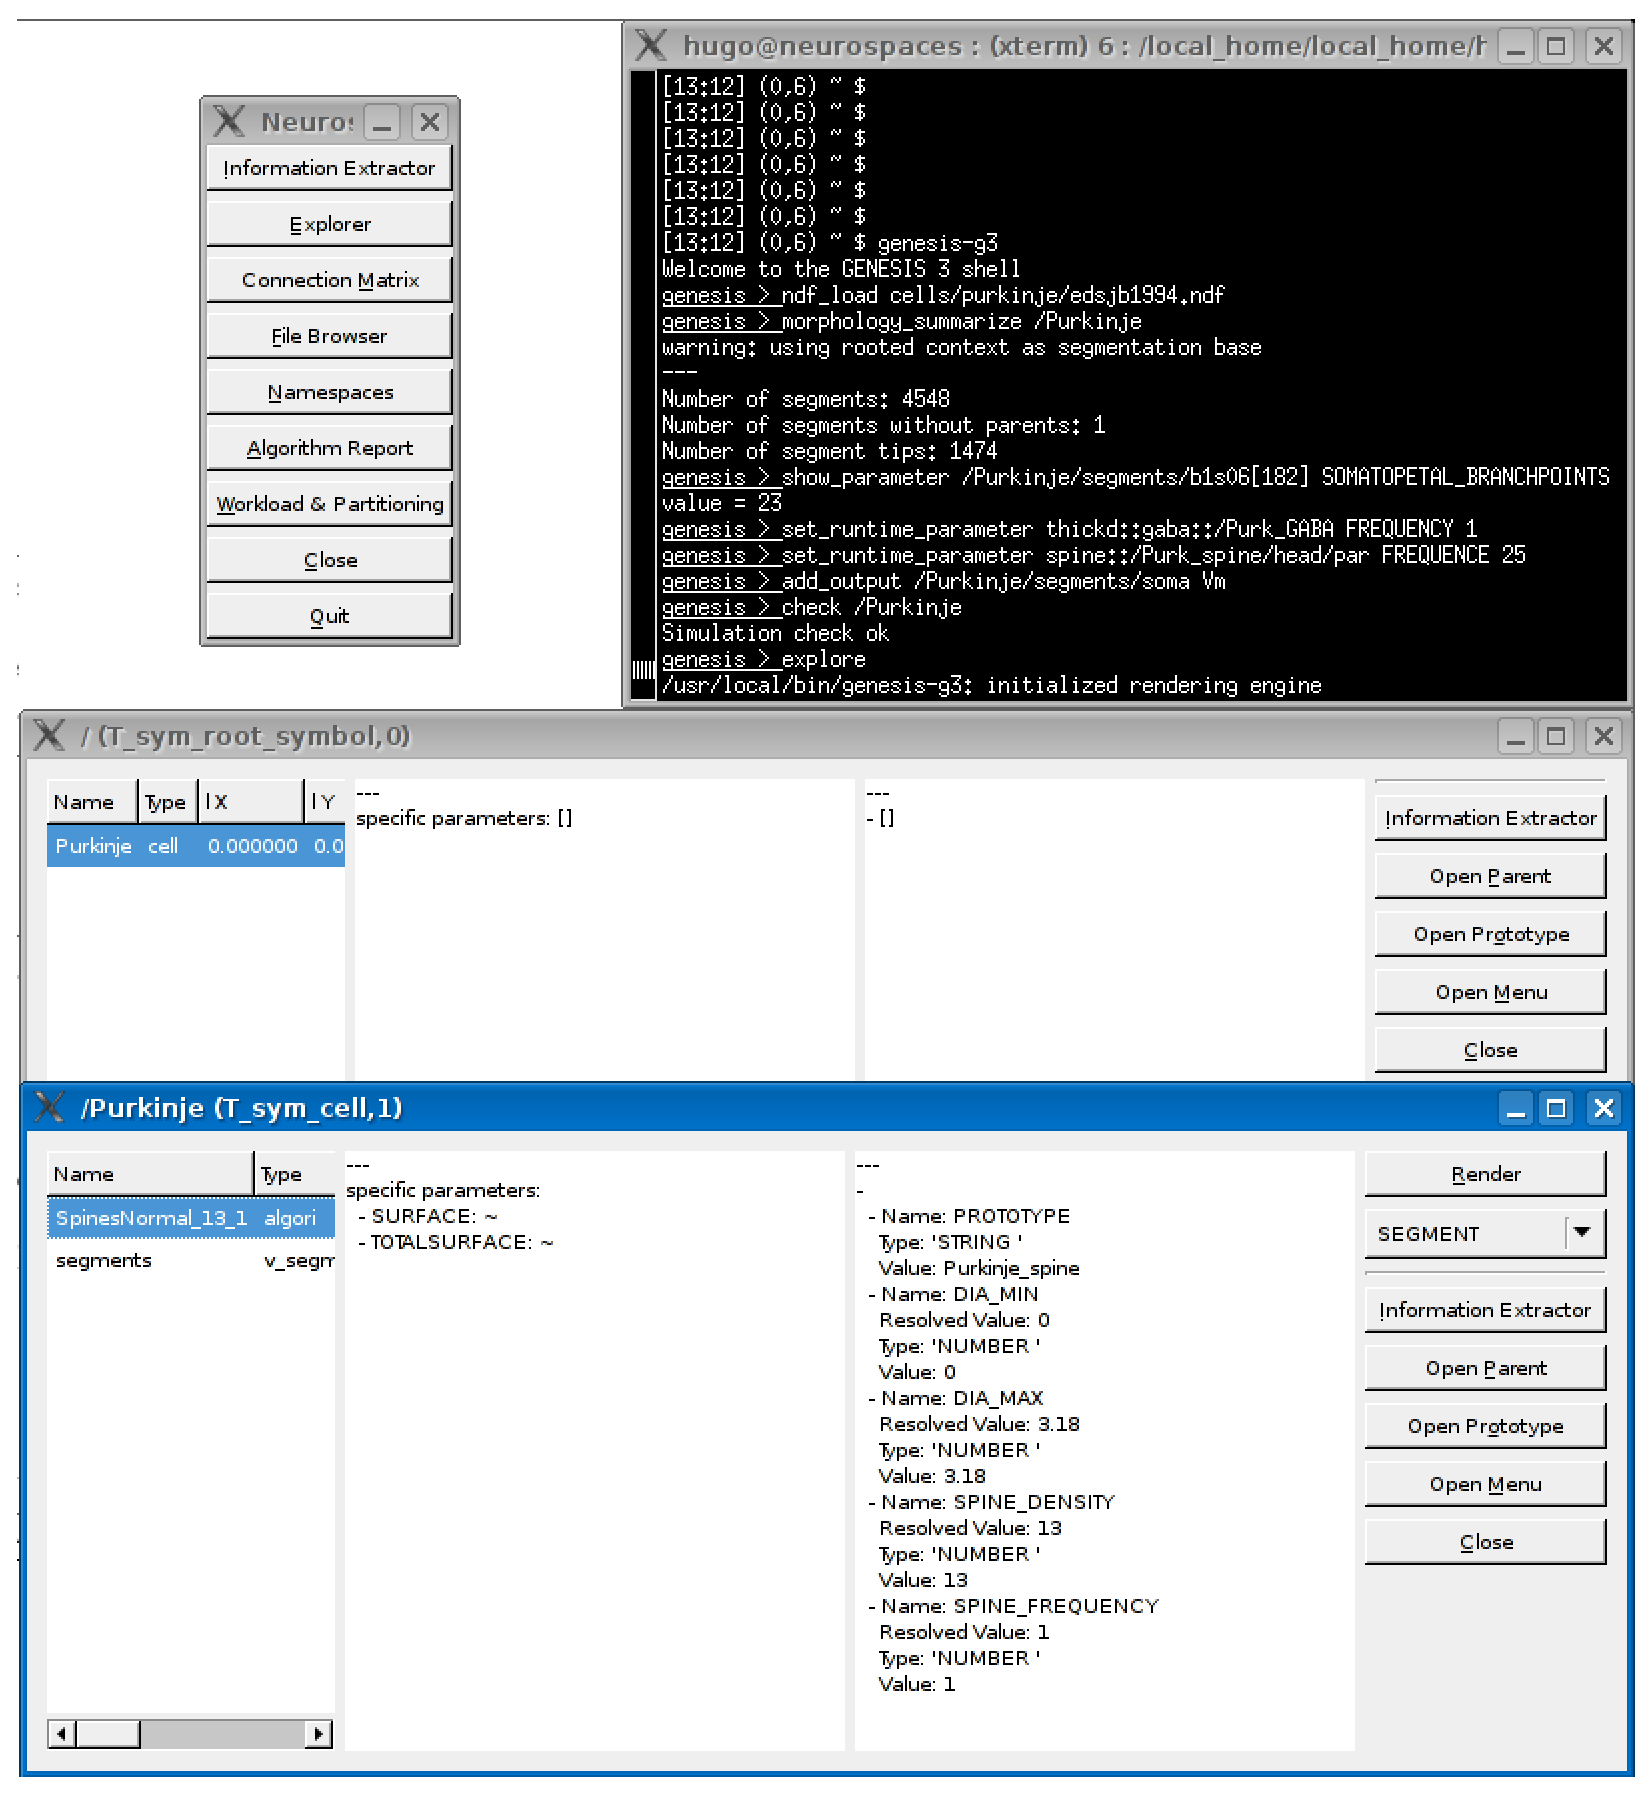
\includegraphics[width=4in]{figures/studio-screenshot.eps}
  \end{center}
  \caption{ {\bf Querying a model in GENESIS 3.0.} The {\bf Studio} is
    a component of the reconfigured GENESIS software platform. It can
    be used to query the parameters of individual compartments in a
    multi-compartment model neuron. The {\bf Studio} also renders 3D
    morphology of dendrites and generates overviews of network models.
  }
  \label{fig:cbi-studio}
\end{figure}

Figure~\ref{fig:cbi-studio} shows sample output of running this
command.  Other capabilities of the {\bf Studio} include rendering
morphologies in three dimensions and generating overviews of network
models (not shown).  In the next section we explore some of the more
graphical capabilities of G-3.


\subsection{Simple Scripting with a CBI Compliant Simulator}
\label{ss-apens}

Python uses modules to group related functions.  G-3 employs Python's
module system to group functions that provide an interface to each of
its software components.
%G-3 scripting
%bindings use modules to separate interfaces for simple models with
%many default settings (e.g. to start a new research project) from more
%complicated interfaces that expose the full functionality of the
%simulator.
As an example, the G-3 Python module {\it nmc} contains functions to
simplify the storage of neuron models in computer memory.  This module
is a simple front-end to the {\bf Model Container}, a G-3 component
which for efficiency is coded in the system programming language C.
Likewise, {\it Heccer} is a wrapper module for the {\bf Heccer}
component which in turn is an interface to a low-level single neuron
solver written in C.  Python bindings for the {\bf Discrete Event System} to facilitate network modeling also exist.

Here we show a simple high-level Python script that runs a simulation of a single cylindrical segment. It
is defined by standard values for the parameters of membrane
resistance ({\tt RM}), axial resistance ({\tt RA}), and membrane
capacitance ({\tt CM}). (Note: This script
  is written for clarity of presentation rather than compactness or
  efficiency. Python version 2.6.6 is used on Linux Ubuntu 10.10
  Maveric.)
%\footnote{The solver requires {\tt RA} for all
%  compartments.}
These parameters are given by their specific values (in SI units) as
commonly reported in the literature, instead of their actual values
scaled to the compartment surface area as used by a mathematical
solver \cite{cornelis04:_neuros_param_handl}. The script defines a
Python function {\it run\_simulation} that will load and run a model when invoked from
a system command line on an appropriately configured computer.  The script
can also be imported into G-3 as a Python module, thus allowing access
to this function.  For convenience, we call this Python module {\it
  example}.

\begin{verbatim}
"""
Comment: Python script running a simple model with G-3.
"""
from g3.nmc import ModelContainer

def RunSimulation(simulationTime):
    timeStep = 1e-5
    
#------------------------------------------------------------------------------
# Create a model container with a neuron cell and a dendritic segment
#------------------------------------------------------------------------------
    my_nmc = ModelContainer()
    my_cell = my_nmc.CreateCell("/cell")
    my_segment = my_nmc.CreateSegment("/cell/soma")

    my_segment.SetParameters(
        {
        "Vm_init": -0.0680,
        "RM": 1.000,
        "RA": 2.50,
        "CM": 0.0164,
        "ELEAK": -0.0800,
        "DIA": 2e-05,
        "LENGTH": 4.47e-05,
        }
        )

# Apply current injection to the soma
    my_segment.SetParameter("INJECT", 1e-9)

#------------------------------------------------------------------------------
# Create a Heccer for computing the neuron model stored by the model container.
#------------------------------------------------------------------------------
    from g3.heccer import Heccer
    my_heccer = Heccer(name="/cell", model=my_nmc)
    my_heccer.CompileAll()

#----------------------------------------------------------------------------- 
# Create an output object.
#------------------------------------------------------------------------------
    from g3.experiment.output import Output
    my_output = Output("/tmp/output")

#----------------------------------------------------------------------------- 
# Link the output object to the address of the computed variable of interest.
#------------------------------------------------------------------------------
    my_output.AddOutput("output", my_heccer.GetAddress("/cell/soma", "Vm"))

#----------------------------------------------------------------------------- 
# Create an array of the objects that participate in the simulation.
#------------------------------------------------------------------------------
    schedulees = []

    # schedule heccer
    schedulees.append(my_heccer)
    schedulees.append(my_output)

#----------------------------------------------------------------------------- 
# Advance all the particpating objects for the duration of the simulation.
#------------------------------------------------------------------------------
    currentTime = 0.0
    while currentTime < simulationTime:
        currentTime += timeStep

        for schedulee in schedulees:
            schedulee.Advance(currentTime)

    my_heccer.Finish()
    my_output.Finish()
  
#------------------------------------------------------------------------------
# Main program executes a simulation of 0.5 seconds.
# The if statement allows use of this file as an executable or as a library.
#------------------------------------------------------------------------------

if __name__ == '__main__':
    RunSimulation(0.5)
\end{verbatim}

%# Second Example: use a wildcard to activate endogenous synapses (see text)
%#    my_nmc.Query("setparameter spine::/Purk_spine/head/par 25")
%#    my_nmc.Query("setparameter thickd::gaba::/Purk_GABA 1")


\subsection{Scripting Chemesis-3}

- Chemesis CNS report.

Our goal was to implement and run two of the G-2 Chemesis tutorial examples.

The example script *cal1.g* creates a single compartment with interaction
between calcium and a buffer.  A second example *cal2.g* creates a two
compartment model with a dendrite and soma. One additional diffusion object
is required to allow for diffusion between compartments.

The two listings below show the G-2 SLI language script *cal1.g* and the G-3
{\bf NDF} representation *cal1.ndf*, found with *cal2.ndf* in
'/usr/local/neurospaces/models/library/chemesis'.


**cal1.ndf**::

\begin{verbatim}
#!neurospacesparse
// -*- NEUROSPACES -*-
NEUROSPACES NDF
// VERSION 0.1
PUBLIC_MODELS
  KINETICS cal1
    PARAMETERS
      PARAMETER ( DIA = 24e-4 ),
      PARAMETER ( LENGTH = 24e-4 ),
    END PARAMETERS
    POOL somaCa
      BINDABLES
        OUTPUT concen
      END BINDABLES
      PARAMETERS
        PARAMETER ( concen_init = 0.001 ),
        PARAMETER ( DIA =  ..->DIA ),
        PARAMETER ( LENGTH =  ..->LENGTH ),
        PARAMETER ( "UNITS" = 1e-3 ),
      END PARAMETERS
    END POOL
    POOL somaCabuf
      BINDABLES
        OUTPUT concen
      END BINDABLES
      PARAMETERS
        PARAMETER ( concen_init = 0.003 ),
        PARAMETER ( DIA =  ..->DIA ),
        PARAMETER ( LENGTH =  ..->LENGTH ),
        PARAMETER ( "UNITS" = 1e-3 ),
      END PARAMETERS
    END POOL
    POOL somabuf
      BINDABLES
        OUTPUT concen
      END BINDABLES
      BINDINGS
        INPUT ../somaCabuf->concen,
      END BINDINGS
      PARAMETERS
        PARAMETER ( concen_init = 0.153 ),
        PARAMETER ( concen_total = 0.153 ),
        PARAMETER ( DIA =  ..->DIA ),
        PARAMETER ( LENGTH =  ..->LENGTH ),
      END PARAMETERS
    END POOL
    REACTION somacabufrxn
      BINDABLES
        INPUT concen, OUTPUT concen
      END BINDABLES
      BINDINGS
                    INPUT ("substrate") ../somaCa->concen,
        INPUT ("substrate") ../somabuf->concen,
        INPUT ("product") ../somaCabuf->concen,
      END BINDINGS
      PARAMETERS
        PARAMETER ( FORWARD_RATE = 1e2 ),
        PARAMETER ( BACKWARD_RATE = 0.5 ),
      END PARAMETERS
    END REACTION
  END KINETICS
END PUBLIC_MODELS
\end{verbatim}


The commands below illustrate how the G-3 Studio (model explorer) is used
to load  *cal1.ndf* into the Model Container and explore the model::

\begin{verbatim}
  \$ genesis-g3
  Welcome to the GENESIS 3 shell
  genesis > ndf_load /usr/local/neurospaces/models/library/chemesis/cal1.ndf
  genesis > explore
\end{verbatim}

[chemesis-cal1.png - sent by Hugo]
[chemesis-cals.png - sent by Hugo]

[if possible -  G-shell commands to run cal1.ndf and output to a file]



\subsection{Multiscale Scripting}

The details of the procedure followed can be seen in the online
documentation "G-3 Extension" (genesis-extend-functionality) and
"chemesis-3-log".


Different numerical solution methods are required to solve the different
types of mathematical equations associated with different scales of
modeling.  The cable equation and ion currents are numerically solved with
implicit Crank-Nicolson integration.  In G-3 this method of solution is
implemented in a dedicated compartmental solver called Heccer.  In the G-3
shell the user has to create a mapping from the name of the neuron model to
the solver.  In the past, this was not necessary, as Heccer was the only
solver.  Under planned extensions to the G-shell syntax, the correct syntax
for a loaded single neuron model with name "/traub94" would be::

\begin{verbatim}
  genesis > solverset "/traub94 => heccer"
\end{verbatim}

Biochemical pathways in neuronal modeling are complex networks of
interacting ion concentration pools.  The G-3 implementation for
simulation of biochemical pathways is called Chemesis-3 and has a
dedicated optimized implementation to represent networks parameterized
with biochemical pathways.  To simulate a complex network model of
biochemical pathways, in this example called "/cal1", a user would
typically type from the G-3 shell::

\begin{verbatim}
  genesis > solverset "/cal1 => chemesis3"
\end{verbatim}

In case the network of biochemical pathways is defined inside the
single neuron model, a user would have to type two commands with
wildcards that associate the correct solver with each component of the
model, for example::

\begin{verbatim}
  genesis > solverset "/**/cal1 => chemesis3"
  genesis > solverset "/traub94/**[!cal1] => heccer"
\end{verbatim}

In later version of G-3 these rules will be built in but still allow
the user to select a different method of solution for different
components of his or her model.


* VERY brief list of steps or description of steps to convert chemesis

  1. Creating a new component "chemesis3"

  2. Creating a new object within an existing "chemesis3".
     "model-container", or "experiment" module

  [Hugo, I will need some help here.  This can be very short, although
  we had originally meant it to be a major part.  Perhaps the first item
  can be glossed over for this audience.]

\subsection{Multi-scale modeling support in G-3}

Supported types by the model-container:

- Grid3D / Populations / Networks

- VolumeConnect / Individual Connections

- Single Cells / Morphology

- HH - Channels / Synaptic (NMDA / AMPA) Channels

- Reaction -- Diffusion


Available solvers, starting at the highest scale:

- DES: discrete event queuing and distribution

- Heccer: single neuron solver.

- Chemesis-3: simple reaction-diffusion systems,

- Experiment: current injections, time-tables and output.


%\begin{figure}[h]
%  \centering
%   
\includegraphics[scale=0.5]{figures/dummyfig.eps}
%\caption{{\bf A Dummy Figure:} Example of \LaTeX\,\,\,code to incorporate a figure into documentation.}
%  \label{fig:df-2}
%\end{figure}

\bibliographystyle{plain}
\bibliography{../tex/bib/g3-refs.bib}

\end{document}
